\section{ Una cuerda como ejemplo en una dimensión }

\begin{center}
    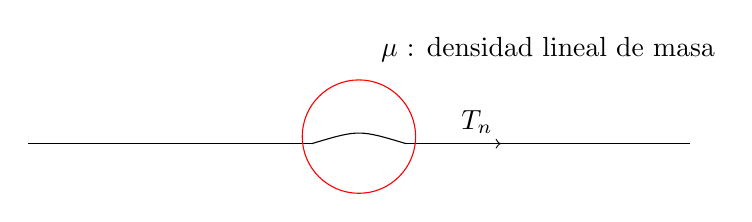
\begin{tikzpicture}[scale=0.6,]
        \draw (-5,0) -- (1,0);
        \draw (1,0) .. controls (2,0.3) .. (3,0);
        \draw (3,0) -- (9,0);
        \draw[ -> ] (4,0) -- (5,0) node [midway, above] {$\vecc{T_n}$};
        \draw (6,2) node {$\mu$ : densidad lineal de masa};

        \draw[color=red] (2, 0.15) circle (1.2);
    \end{tikzpicture}
\end{center}

Considerando el pedazo de cuerda afectado por la deformación,
la cual suponemos como pequeña. Consideramos como deformación
pequeña aquella en la que, con el diagrama de abajo,

\(\theta_{1,2} \approx 0 \land \sin(\theta_{1,2}) \approx \tan(\theta_{1,2})\)

\begin{center}
    \begin{tikzpicture}
        \begin{axis}[
                axis lines = center,
                xlabel = \(X\),
                ylabel = \(Y\),
                xmin = 0,
                xmax = 10,
                ymin = 0,
                ymax = 2,
                xtick = {0},
                ytick = {0},
                width=0.8\textwidth,
                height=0.5\textwidth,
                clip=false,
            ]
                \addplot[
                    domain=0:2*pi,
                    samples = 100,
                ]{
                    sin(deg(0.5*x))
                };
                \addplot[
                    domain=2:3,
                    samples = 100,
                    color=blue,
                    thick
                ]{
                    sin(deg(0.5*x))
                };
                            
                \draw[ -> ] (3,0.997494987) -- (4.5, 1.05054788) 
                    node [midway, above] {$\vecc{T_{n,2}}$};
                \draw[ dotted ] (4.5, 1.05054788) -- (7, 1.138969390);
                \draw[ dotted ] (3,0.997494987) -- (7,0.997494987);
                \coordinate (A) at (6, 1.103600789);
                \coordinate (B) at (3,0.997494987);
                \coordinate (C) at (6, 0.997494987);

                \pic [
                    draw,
                    -,
                    black,
                    angle eccentricity=1.3,
                    angle radius=3cm,
                    "$\theta_2$"]
                    {angle = C--B--A};
                
                \draw[ -> ] (2, 0.841470985) -- (0.5, 0.436244255)
                    node [midway, below=6pt, xshift=5pt] {$\vecc{T_{n,1}}$};
                \draw[ dotted] (2, 0.841470985) -- (0.5, 0.841470985);

                \coordinate (D) at (0.5, 0.841470985);
                \coordinate (E) at (2, 0.841470985);
                \coordinate (F) at (0.5, 0.436244255);

                \pic [
                    draw,
                    -,
                    black,
                    angle eccentricity=1.3,
                    angle radius=1cm,
                    "$\theta_1$"]
                    {angle = D--E--F};

                    \draw[ dotted ] (2,0) -- (E);
                    \draw (2,0) -- (2, -0.1) node[below] {$x^*$};
                    \draw[ dotted ] (3,0) -- (B); 
                    \draw (3,0) -- (3, -0.15) node[below, xshift=10pt] {$x^* + \Delta x^*$};
                    \draw (2.5, 1.1) node {$\Delta m$};
                    \draw (2.5, 0.8) node {$\Delta s$};
                    
            \end{axis}
            
    \end{tikzpicture}
\end{center}